就像计算机网络中分层的概念一样,\textbf{对于某一层次的观察者来说,观察者只需关注此层的一些概念,不用理会下层是如何工作和实现的。}同理,现代计算机也不是一种简单的电子设备,而是由硬件与软件结合而成的复杂整体。它通常由\textbf{5个不同的层次组成},在每一层上都能够进行程序设计,如图1-7所示。

\textbf{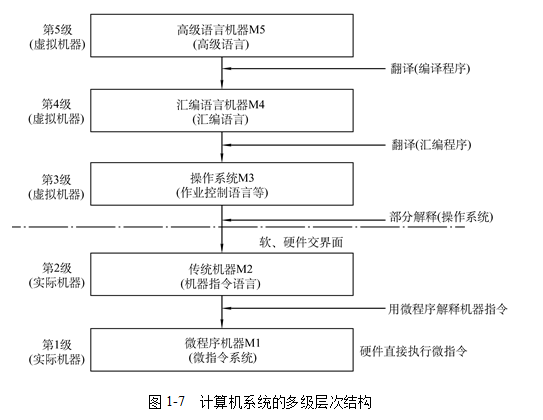
\includegraphics[width=3.70833in,height=2.86458in]{png-jpeg-pics/CDBD5A691A94AEC34E2EBAA37A85F095.png}}

\textbf{}

\textbf{{补充知识点:编译程序、解释程序、汇编程序的区别。}}

解析:汇编程序是用汇编语言编写的程序,与编译程序、解释程序完全不是一个概念。

\textbf{总结:}

\textbf{1)}解释程序是高级语言翻译程序的一种,它将源语言书写的源程序作为输入,解释一句就提交给计算机执行一句,并不形成目标程序。

\textbf{2)}编译程序把高级语言源程序作为输入,进行翻译转换,产生出机器语言的目标程序,然后让计算机去执行这个目标程序,得到计算结果。
